%Input preamble
%Style
\documentclass[12pt]{article}
\usepackage[top=1in, bottom=1in, left=1in, right=1in]{geometry}
\parindent 22pt
\usepackage{fancyhdr}

%Packages
\usepackage{adjustbox}
\usepackage{amsmath}
\usepackage{amsfonts}
\usepackage{amssymb}
\usepackage[english]{babel}
\usepackage{bm}
\usepackage[table]{xcolor}
\usepackage{tabu}
\usepackage{color,soul}
\usepackage[utf8x]{inputenc}
\usepackage{makecell}
\usepackage{longtable}
\usepackage{multirow}
\usepackage[normalem]{ulem}
\usepackage{etoolbox}
\usepackage{graphicx}
\usepackage{tabularx}
\usepackage{ragged2e}
\usepackage{booktabs}
\usepackage{caption}
\usepackage{fixltx2e}
\usepackage[para, flushleft]{threeparttablex}
\usepackage[capposition=top]{floatrow}
\usepackage{subcaption}
\usepackage{pdfpages}
\usepackage{pdflscape}
\usepackage[sort&compress]{natbib}
\usepackage{bibunits}
\usepackage[colorlinks=true,linkcolor=darkgray,citecolor=darkgray,urlcolor=darkgray,anchorcolor=darkgray]{hyperref}
\usepackage{marvosym}
\usepackage{makeidx}
\usepackage{setspace}
\usepackage{enumerate}
\usepackage{rotating}
\usepackage{epstopdf}
\usepackage[titletoc]{appendix}
\usepackage{framed}
\usepackage{comment}
\usepackage{xr}
\usepackage{titlesec}
\usepackage{footnote}
\usepackage{longtable}
\newlength{\tablewidth}
\setlength{\tablewidth}{9.3in}
\usepackage[bottom]{footmisc}
\usepackage{stackengine}
\newcommand\barbelow[1]{\stackunder[1.2pt]{$#1$}{\rule{1ex}{.085ex}}}
\usepackage{titletoc}
\usepackage{accents}
\usepackage{arydshln }
\usepackage{titletoc}
\titlespacing{\section}{.2pt}{1ex}{1ex}
\setcounter{section}{0}
\renewcommand{\thesection}{\arabic{section}}


\makeatletter
\pretocmd\start@align
{%
  \let\everycr\CT@everycr
  \CT@start
}{}{}
\apptocmd{\endalign}{\CT@end}{}{}
\makeatother
%Watermark
\usepackage[printwatermark]{xwatermark}
\usepackage{lipsum}
\definecolor{lightgray}{RGB}{220,220,220}
\definecolor{dimgray}{RGB}{105,105,105}

%\newwatermark[allpages,color=lightgray,angle=45,scale=3,xpos=0,ypos=0]{Preliminary Draft}

%Further subsection level
\usepackage{titlesec}
\titleformat{\paragraph}
{\normalfont\normalsize\bfseries}{\theparagraph}{1em}{}
\titlespacing*{\paragraph}
{0pt}{3.25ex plus 1ex minus .2ex}{1.5ex plus .2ex}

\titleformat{\subparagraph}
{\normalfont\normalsize\bfseries}{\thesubparagraph}{1em}{}
\titlespacing*{\subparagraph}
{0pt}{3.25ex plus 1ex minus .2ex}{1.5ex plus .2ex}

%Functions
\DeclareMathOperator{\cov}{Cov}
\DeclareMathOperator{\sign}{sgn}
\DeclareMathOperator{\var}{Var}
\DeclareMathOperator{\plim}{plim}
\DeclareMathOperator*{\argmin}{arg\,min}
\DeclareMathOperator*{\argmax}{arg\,max}

%Math Environments
\usepackage{amsthm}
\newtheoremstyle{mytheoremstyle} % name
    {\topsep}                    % Space above
    {\topsep}                    % Space below
    {\color{black}}                   % Body font
    {}                           % Indent amount
    {\itshape \color{dimgray}}                   % Theorem head font
    {.}                          % Punctuation after theorem head
    {.5em}                       % Space after theorem head
    {}  % Theorem head spec (can be left empty, meaning ?normal?)

\theoremstyle{mytheoremstyle}
\newtheorem{assumption}{Assumption}
\renewcommand\theassumption{\arabic{assumption}}

\theoremstyle{mytheoremstyle}
\newtheorem{assumptiona}{Assumption}
\renewcommand\theassumptiona{\arabic{assumptiona}a}

\newtheorem{assumptionb}{Assumption}
\renewcommand\theassumptionb{\arabic{assumptionb}b}

\newtheorem{assumptionc}{Assumption}
\renewcommand\theassumptionc{\arabic{assumptionc}c}

\theoremstyle{mytheoremstyle}
\newtheorem{lemma}{Lemma}

\theoremstyle{mytheoremstyle}
\newtheorem{proposition}{Proposition}

\theoremstyle{mytheoremstyle}
\newtheorem{corollary}{Corollary}

%Commands
\newcommand\independent{\protect\mathpalette{\protect\independenT}{\perp}}
\def\independenT#1#2{\mathrel{\rlap{$#1#2$}\mkern2mu{#1#2}}}
\newcommand{\overbar}[1]{\mkern 1.5mu\overline{\mkern-1.5mu#1\mkern-1.5mu}\mkern 1.5mu}
\newcommand{\equald}{\ensuremath{\overset{d}{=}}}
\captionsetup[table]{skip=10pt}
%\makeindex

%Table, Figure, and Section Styles
\captionsetup[figure]{labelfont={bf},name={Figure},labelsep=period}
\renewcommand{\thefigure}{\arabic{figure}}
\captionsetup[table]{labelfont={bf},name={Table},labelsep=period}
\renewcommand{\thetable}{\arabic{table}}
\titleformat{\section}{\centering \normalsize \bf}{\thesection.}{0em}{}%\titlespacing*{\subsection}{0pt}{0\baselineskip}{0\baselineskip}
\renewcommand{\thesection}{\arabic{section}}

\titleformat{\subsection}{\flushleft \normalsize \bf}{\thesubsection}{0em}{}
\renewcommand{\thesubsection}{\arabic{section}.\arabic{subsection}}

%No indent
\setlength\parindent{24pt}
\setlength{\parskip}{5pt}

%Logo
%\AddToShipoutPictureBG{%
%  \AtPageUpperLeft{\raisebox{-\height}{\includegraphics[width=1.5cm]{uchicago.png}}}
%}

\newcolumntype{L}[1]{>{\raggedright\let\newline\\\arraybackslash\hspace{0pt}}m{#1}}
\newcolumntype{C}[1]{>{\centering\let\newline\\\arraybackslash\hspace{0pt}}m{#1}}
\newcolumntype{R}[1]{>{\raggedleft\let\newline\\\arraybackslash\hspace{0pt}}m{#1}} 

\newcommand{\mr}{\multirow}
\newcommand{\mc}{\multicolumn}

%\newcommand{\comment}[1]{}

\begin{document}


\title{\Large \textbf{Does Entrepreneurship Mitigate or Exacerbate Social Mobility? }}
\author{Yi Ling}

\date{\today}

\maketitle

\thispagestyle{empty} 
\doublespacing
\thispagestyle{empty} 

\section{Research Question}
This proposal aims to compare the outcomes of two types of entrepreneurs:  nascent entrepreneurs and entrepreneurs whose family is also self-employed, and examine whether the first type faces lower intergenerational mobility than the second type, in other words, can people from a non-entrepreneur family background climb up the social ladder through choosing to start a business?

\section{Literature Review}
This research explores the link between entrepreneurship and intergenerational mobility, whether choosing to be an entrepreneur will increase intergenerational mobility. The first relates to the entrepreneurship's impact on wealth concentration and inequality. \citet{quadrini1999importance} points out that entrepreneurship has implications for high wealth concentration: entrepreneurs have higher asset holdings even though their income is not larger than non-entrepreneurs. Moreover, entrepreneurs have greater upward mobility, which means they have a greater probability of moving to higher wealth classes, and this is not only due to their higher incomes. \citet{cagetti2006entrepreneurship} also emphasizes that the reason why entrepreneurs have higher wealth is because they save more for borrowing constraints, and share the fortune with their children to keep the family firm working. This research aims to find whether the saving patterns of two types of entrepreneurs are different, which leads to the high saving rate of entrepreneurs.


The second relates to the literature on social mobility. Intergenerational mobility has long been a central topic of interest for economists worldwide, as greater inequality in a society tends to make family background a stronger determinant of offspring’s outcomes \citep{corakIncomeInequalityEquality2013a}. There are many discussions on how parental self-employment impacts children's occupation decisions \citep{dunn2000financial, laferrere2001self, djankov2006china, barnir2011parental, lindquist2015entrepreneurial}. This research is most closely related to \citet{barnir2011parental, lindquist2015entrepreneurial}. \citet{barnir2011parental} compare first-generation self-employers and self-employers who have entrepreneurial parents, they found that through vicarious learning, people who have entrepreneurial parents can observe and learn from their family, which makes it easier to become an entrepreneur, but they face the same financial constraints when their firm enters the market.  \citet{lindquist2015entrepreneurial} also compares the difference between the entrepreneurs whose parents were self-employed and those whose parents were not, they found that parental entrepreneurship increases the probability of children’s entrepreneurship by about 60\% due to role modeling.  Other papers consider the occupation decision within the entrepreneur family. \citet{dunn2000financial, laferrere2001self, djankov2006china} found offspring of the self-employed display a greater propensity to become entrepreneurs. Previous literature also explores the intergenerational mobility in many other aspects \citep{peters1992patterns, checchi1999more}. For instance, \citet{chetty2018impacts} analyzes the neighborhood's impact on intergenerational mobility, finding out the outcome of the children is better when they spend their childhood in better opportunity areas.


The third relates to the macroeconomic and public literature on determinants of entrepreneurship and entrepreneurial returns. Since the returns of two types of entrepreneurs might be different, this might be the reason why entrepreneurial returns are lower than workers. The classic puzzle in macroeconomics is the "Private Equity Premium Puzzle", which means entrepreneurs have lower returns than public equity returns \citep{moskowitz2002returns, bhandari2020survey}. Since they have lower returns, the reasons why people choose to be entrepreneurs are widely discussed \citep{parker2005economics, vereshchagina2009risk}. \citet{parker2005economics} summarizes these reasons and adds other explanations: the risk of entrepreneurs' net worth is less than the risk of business, and entrepreneurs could tolerate the high risk in their businesses. Additionally, \citet{vereshchagina2009risk} suggested that non-concavity areas created in the interaction with an occupational choice between being an entrepreneur and an employee could explain the high risk in investment. This research also aims to calculate the returns of two types of entrepreneurial investment. If first-generation entrepreneurs earn lower returns while those with parental self-employment backgrounds earn higher returns, then the apparent puzzle can be explained by the higher failure rate among first-generation entrepreneurs. 

\section{Data Description}
There are many data sources that provide information on income, profits, and investments for entrepreneurs and their family backgrounds. One prominent dataset is the Panel Study of Income Dynamics (PSID), a longitudinal household survey that began in 1968 and covers a nationally representative sample of over 18,000 individuals from 5,000 families in the United States. \citet{quadrini1999importance,fairlie1999absence} both use the  (PSID) to study the financial and human capital transition across generations. 

The second dataset is the Current Population Survey (CPS), which is an important source of labor force data in the United States. To study the entrepreneurship trend, \citet{jiang2023skill, sanchez2023decline, bento2023barriers} both used CPS and found the decline trend in the entrepreneur population. Before calculating the income, investment of two types of entrepreneurs, I also calculated the population trend to ensure my definition of entrepreneurs is the same as previous literature. First, I only included the people who have an active employment status. Second, I define entrepreneurs as "self-employed" from the data. For family background, I only consider parents' employment status first, then I merge parents' employment information with the original data. Figure \ref{nascent} shows the population trend of nascent entrepreneurs, which is consistent with the results from \citet{jiang2023skill, sanchez2023decline}.

\begin{figure}[htp!]
    \centering
    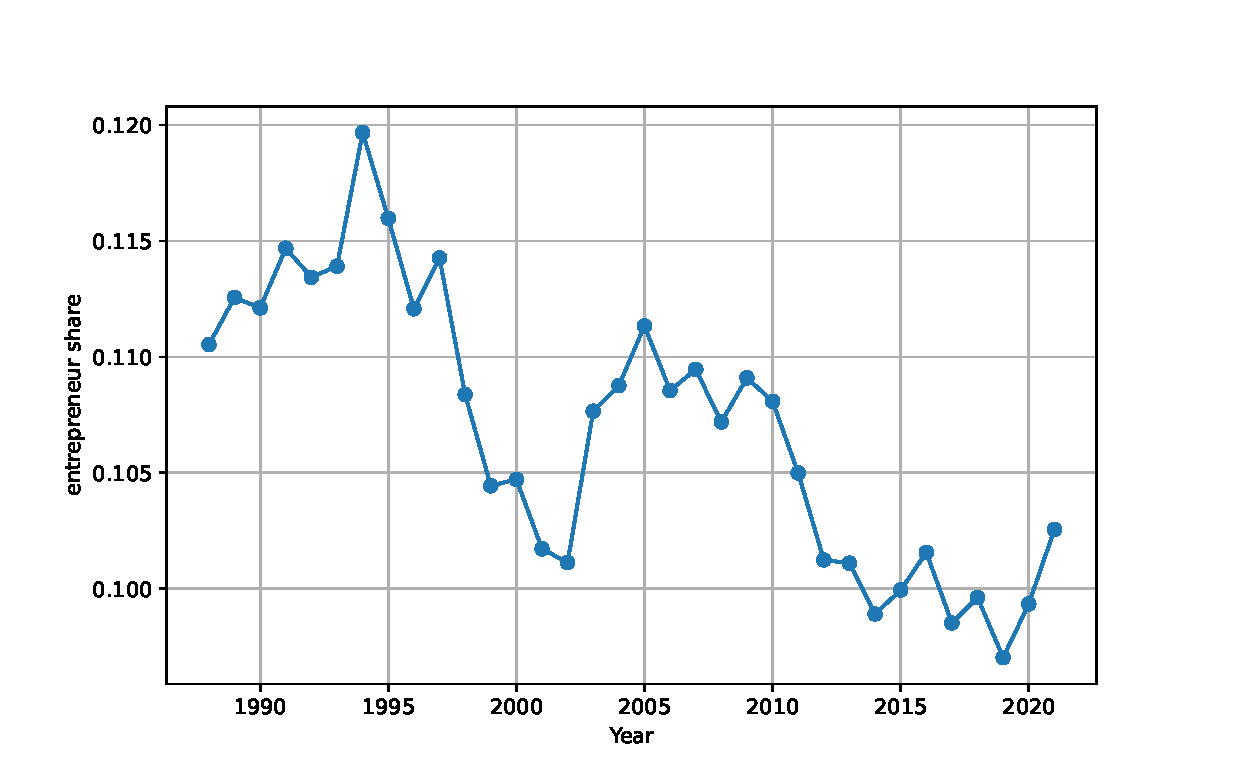
\includegraphics[width=0.5\textwidth]{nascententrepreneursharecps.eps}
    \caption{Population Trend of Nascent Entrepreneurs}
    \label{nascent}
\end{figure}


Another dataset is also helpful to identify the entrepreneur trend over time, but it cannot provide detailed information about the entrepreneurs' families. For instance, Survey of Consumer Finance (SCF) is also widely used to observe the entreprenuers population and investment \citep{moskowitz2002returns, cagetti2006entrepreneurship}, however, the question in the inverview is " How did you (or your family living here) first acquire this business; was it bought or invested in, started by you,  inherited, given to you, or some other way?", therefore, we cannot identify whether the business is started by that person or his family.

\section{Empirical Design}

The two-way fixed effect model is designed to identify the returns in different groups. First, we need to define the returns of entrepreneurs, which are the returns of capital gains from the business, on the equity. Therefore, we need to identify both capital gains and equity precisely. Since  \citep{moskowitz2002returns} calculates the returns using the Survey of Consumer Finance, we can identify both capital gains and equity in the same logit using PSID as well. Since PSID provides both business income (profits) and labor income (wages), and is consistent with \citep{moskowitz2002returns}, we can also consider retained earnings as the ratio $\gamma$ of the profits. The capital gain is calculated in this way:

\begin{equation}
    Capital\ Gain _{t}=Profits _{t} (1-\gamma )-Wage _{t}
    \label{capital_gain}
\end{equation}

PSID also provides much information about the household head's wealth, which includes assets, stocks, and other real estate. Denote that we have $K$ types of assets, the equity of the entrepreneur $i$ in time $t$ is:

\begin{equation}
    Equity _{t}= \sum_{k=1}^{k=K} Assets _{ikt} 
    \label{market_value}
\end{equation}

For workers, since salary is the only source of income, we calculate the returns of wages on equity, $\lambda_t$ and $\theta_i$ control time fixed effect and individual fixed effect, and $W_{it}$ control workers' education level and age, the baseline model is:

\begin{equation}
	Equity_{it}= \alpha_0+\alpha_1 Wage_{it}+\lambda_t+\theta_i+W_{it}+\eta_{it}
\end{equation}

Then, we should control for individual fixed effects $\iota_i$, since different types of firms might lead to different revenue. For example, technology companies tend to have higher revenue than manufacturing firms. Moreover, we should control for time fixed effects $\gamma_t$, since the monetary and fiscal shocks that happened in certain years might affect the revenue for all of the firms. Moreover, denote $SelfEmployed_{it}$ as a dummy variable whether this household head's parents are self-employed or not. $X_{it}$ denotes other variables that we should control, including education level, age of the entrepreneurs. Finally, two way the two-way fixed effect model is set up:
 \begin{equation}
    Equity_{it}= \beta_0+\beta_1 CapitalGain_{it}+\beta_2 CapitalGain_{it}* SelfEmployed_{it}+\gamma_t+\iota_i+X_{it}+\epsilon_{it}
\end{equation}

\bibliographystyle{apalike} 
\bibliography{references}

\end{document}

